\documentclass{article}
\usepackage{physics}
\usepackage{graphicx}
\usepackage{caption}
\usepackage{amsmath}
\usepackage{bm}
\usepackage{framed}
\usepackage{authblk}
\usepackage{empheq}
\usepackage{amsfonts}
\usepackage{esint}
\usepackage[makeroom]{cancel}
\usepackage{dsfont}
\usepackage{centernot}
\usepackage{mathtools}
\usepackage{subcaption}
\usepackage{bigints}
\usepackage{amsthm}
\theoremstyle{definition}
\newtheorem{lemma}{Lemma}
\newtheorem{defn}{Definition}[section]
\newtheorem{prop}{Proposition}[section]
\newtheorem{rmk}{Remark}[section]
\newtheorem{thm}{Theorem}[section]
\newtheorem{exmp}{Example}[section]
\newtheorem{prob}{Problem}[section]
\newtheorem{sln}{Solution}[section]
\newtheorem*{prob*}{Problem}
\newtheorem{exer}{Exercise}[section]
\newtheorem*{exer*}{Exercise}
\newtheorem*{sln*}{Solution}
\usepackage{empheq}
\usepackage{tensor}
\usepackage{xcolor}
%\definecolor{colby}{rgb}{0.0, 0.0, 0.5}
\definecolor{MIT}{RGB}{163, 31, 52}
\usepackage[pdftex]{hyperref}
%\hypersetup{colorlinks,urlcolor=colby}
\hypersetup{colorlinks,linkcolor={MIT},citecolor={MIT},urlcolor={MIT}}  
\usepackage[left=1in,right=1in,top=1in,bottom=1in]{geometry}
\setcounter{MaxMatrixCols}{20}
\usepackage{newpxtext,newpxmath}
\newcommand*\widefbox[1]{\fbox{\hspace{2em}#1\hspace{2em}}}

\newcommand{\p}{\partial}
\newcommand{\R}{\mathbb{R}}
\newcommand{\C}{\mathbb{C}}
\newcommand{\lag}{\mathcal{L}}
\newcommand{\nn}{\nonumber}
\newcommand{\ham}{\mathcal{H}}
\newcommand{\M}{\mathcal{M}}
\newcommand{\I}{\mathcal{I}}
\newcommand{\K}{\mathcal{K}}
\newcommand{\F}{\mathcal{F}}
\newcommand{\w}{\omega}
\newcommand{\lam}{\lambda}
\newcommand{\al}{\alpha}
\newcommand{\be}{\beta}
\newcommand{\x}{\xi}

\newcommand{\G}{\mathcal{G}}

\newcommand{\f}[2]{\frac{#1}{#2}}

\newcommand{\ift}{\infty}

\newcommand{\lp}{\left(}
\newcommand{\rp}{\right)}

\newcommand{\lb}{\left[}
\newcommand{\rb}{\right]}

\newcommand{\lc}{\left\{}
\newcommand{\rc}{\right\}}


\newcommand{\V}{\mathbf{V}}
\newcommand{\U}{\mathcal{U}}
\newcommand{\Id}{\mathcal{I}}
\newcommand{\D}{\mathcal{D}}
\newcommand{\Z}{\mathcal{Z}}

%\setcounter{chapter}{-1}


\usepackage{enumitem}



\usepackage{listings}
\captionsetup[lstlisting]{margin=0cm,format=hang,font=small,format=plain,labelfont={bf,up},textfont={it}}
\renewcommand*{\lstlistingname}{Code \textcolor{violet}{\textsl{Mathematica}}}
\definecolor{gris245}{RGB}{245,245,245}
\definecolor{olive}{RGB}{50,140,50}
\definecolor{brun}{RGB}{175,100,80}

%\hypersetup{colorlinks,urlcolor=colby}
\lstset{
	tabsize=4,
	frame=single,
	language=mathematica,
	basicstyle=\scriptsize\ttfamily,
	keywordstyle=\color{black},
	backgroundcolor=\color{gris245},
	commentstyle=\color{gray},
	showstringspaces=false,
	emph={
		r1,
		r2,
		epsilon,epsilon_,
		Newton,Newton_
	},emphstyle={\color{olive}},
	emph={[2]
		L,
		CouleurCourbe,
		PotentielEffectif,
		IdCourbe,
		Courbe
	},emphstyle={[2]\color{blue}},
	emph={[3]r,r_,n,n_},emphstyle={[3]\color{magenta}}
}

\newcommand{\diag}{\text{diag}}
\newcommand{\psirot}{\ket{\psi_\text{rot}(t)} }
\newcommand{\RWA}{\ham_\text{rot}^\text{RWA}}


\begin{document}
\begin{framed}
\noindent Name: \textbf{Huan Q. Bui}\\
Course: \textbf{8.421 - AMO I}\\
Problem set: \textbf{\#4}\\
Due: Friday, March 5, 2022.
\end{framed}
	
	
\noindent \textbf{1. Sum rule for fine structure}

\begin{enumerate}[label=(\alph*)]
	\item For classical $\vec{L}, \vec{S}$, we simply have
	\begin{align*}
	\langle \vec{L} \cdot \vec{S} \rangle = LS\langle \cos\theta\rangle_\theta  \propto \int_0^{2\pi}\cos\theta\,d\theta = 0
	\end{align*}
	as expected. 
	
	
	\item It turns out that the same thing happens in quantum mechanics, but there are subtleties. $\vec{L}$ and $\vec{S}$ are now operators, and we have
	\begin{align*}
	\vec{L}\cdot \vec{S} = \f{1}{2}\lb (\vec{J} + \vec{S})^2 - \vec{L}^2 - \vec{S}^2\rb = \f{1}{2}(J^2 - L^2 - S^2)
	\end{align*}
	where
	\begin{align*}
	\vec{J} = \vec{L} + \vec{S}.
	\end{align*}
	Note that a more explicit notation for the kets would be $\ket{L,S,J,m_J}$ which has all of the good quantum numbers and suggests that we are working in the $\{J,m_J\}$ basis. From here is it clear that $\ket{J,m_J}$'s are eigenstates of $J^2, L^2,S^2$.   In any case, we have 
	\begin{align*}
	\sum_{J,m_J} \bra{J,m_J} \vec{L}\cdot \vec{S} \ket{J,m_J} 
	&= \f{1}{2}\sum_{J,m_J} \bra{J,m_J} J^2 - L^2 - S^2 \ket{J,m_J}\\
	&= \f{1}{2}\sum_{J,m_J} [J(J+1) - L(L+1) - S(S+1)] \\
	&= \f{1}{2}\sum_{J} \underbrace{\sum_{m_J = -J}^J}_{2J+1 \text{ terms}}[J(J+1) - L(L+1) - S(S+1)] \\
	&= \f{1}{2} \sum_{J=\abs{L-S}}^{\abs{L+S}} (2J+1) [J(J+1) - L(L+1) - S(S+1)].
	\end{align*}
	Just for fun, let us prove this statement directly. Assume without loss of generality that $L\geq S$, so we could drop the absolute value sign to write
	\begin{align*}
	\sum_{J,m_J} \bra{J,m_J} \vec{L}\cdot \vec{S} \ket{J,m_J} = \f{1}{2} \sum_{J={L-S}}^{{L+S}} (2J+1) [J(J+1) - L(L+1) - S(S+1)].
	\end{align*}
	To simplify, let's introduce $J' = J-L$, so that we can write
	\begin{align*}
	\sum_{J,m_J} \bra{J,m_J} \vec{L}\cdot \vec{S} \ket{J,m_J} = \f{1}{2} \sum_{J'={-S}}^{{S}} (2 (J' + L) + 1)[(J' + L) ((J' + L) + 1) - L (L + 1) - S (S + 1)].
	\end{align*}
	Now we take $S = n/2$ where $n\in \mathbb{N}$. We will show that the sum above vanishes by induction on $S$ (not $n$! This is a subtle point.). For $S=0$, the sum is trivially zero (which makes sense since there is no $\vec{S}$ to couple with $\vec{L}$). For $S=1/2$, we can check that the sum is also zero. With these we have covered all base cases. Now let us assume that the sum is zero for $S=N/2$ for some $N\in \mathbb{N}$. We will show that the sum is also zero for $S' = N/2+1$. To this end, we simply calculate:
	\begin{align*}
	\sum_{J,m_J} \bra{J,m_J} \vec{L}\cdot \vec{S}' \ket{J,m_J} 
	&= \f{1}{2} \sum_{J'={-S'}}^{{S'}} (2 (J' + L) + 1)[(J' + L) ((J' + L) + 1) - L (L + 1) - S' (S' + 1)] \\
	&= \f{1}{2} \sum_{J'={-N/2-1}}^{{N/2+1}} (2 (J' + L) + 1)\lb (J' + L) ((J' + L) + 1) - L (L + 1) - \lp \f{N}{2} + 1\rp \lp \f{N}{2} + 1 + 1\rp \rb \\
	&= \f{1}{2} \sum_{J'={-N/2-1}}^{{N/2+1}} (2 (J' + L) + 1)\lb (J' + L) ((J' + L) + 1) - L (L + 1) - \f{N}{2}\lp \f{N}{2} + 1 \rp - 2\lp \f{N}{2} + 1 \rp\rb \\
	\text{(inductive hypothesis)  }&= \f{2 (-N/2-1 + L) + 1}{2}\lb (-N/2-1 + L) ((-N/2-1 + L) + 1) - L (L + 1) - N/2\lp N/2 + 1 \rp\rb \\
	&\quad\quad + \f{2 (N/2+1 + L) + 1}{2}\lb (N/2+1 + L) ((N/2+1 + L) + 1) - L (L + 1) - N/2\lp N/2 + 1 \rp\rb \\
	&\quad\quad + \f{1}{2}\sum_{J'=-N/2-1}^{N/2+1} (2 (J' + L) + 1) \lb -2\lp \f{N}{2}+1 \rp \rb + 0 \\
	&= -L (-1 + 2 L - N) (2 + N) + (1 + L) (2 + N) (3 + 2 L + N) -((1 + 2 L) (2 + N) (3 + N)) \\
	&= 0. 
	\end{align*}
	Therefore, by the principle of induction we have shown that 
	\begin{align*}
	\sum_{J,m_J} \bra{J,m_J} \vec{L}\cdot \vec{S} \ket{J,m_J}  = 0.
	\end{align*}
	Notice that by picking $N$ to be odd and even we can cover all cases. As a result, the sum rule is proved. 
	
	\item  That was tedious! An elegant way to prove the statement above is to notice that 
	\begin{align*}
	\sum_{J,m_J} \bra{J,m_J} \vec{L}\cdot \vec{S} \ket{J,m_J} = \Tr(\vec{L}\cdot \vec{S}).
	\end{align*}
	Since the trace of an operator is invariant under a basis change, we may move to the $\ket{Lm_L S m_S}$ basis: 
	\begin{align*}
	\sum_{J,m_J} \bra{J,m_J} \vec{L}\cdot \vec{S} \ket{J,m_J} &= \Tr(\vec{L}\cdot \vec{S}) \\
	&= \sum_{m_L,m_S} \bra{m_L m_S} \vec{L}\cdot \vec{S} \ket{m_L m_S} \\
	&= \sum_{m_L,m_S} \bra{m_L m_S} L_xS_x+L_yS_y+L_zS_z \ket{m_L m_S} \\
	&= \sum_{m_L,m_S} \bra{m_L m_S} \f{1}{2}(L_+S_- + L_-S_+)   +L_zS_z \ket{m_L m_S} \\
	&= \sum_{m_L,m_S} \bra{m_L m_S} L_zS_z \ket{m_L m_S} \\
	&= \sum_{m_L=-L}^L\sum_{m_S=-S}^S m_L m_S = 0,
	\end{align*} 
	where we have expressed $L_x,L_y,S_x,S_y$ in terms of the associated lowering and raising operators:
	\begin{align*}
	L_x &= \f{1}{2}(L_+ + L_-)\\
	L_y &= \f{1}{2i}(L_+ - L_-)\\
	S_x &= \f{1}{2}(S_+ + S_-)\\
	S_y &= \f{1}{2i}(S_+ - S_-).
	\end{align*}
	And we're done with the proof of the sum rule. 
\end{enumerate}

\noindent \textbf{2. Atoms with two valance electrons: From $LS$-coupling to $jj$-coupling.} We have two atoms with spins $\vec{s}_1,\vec{s}_2$ and angular momenta $\vec{l}_1, \vec{l}_2$. There is the exchange interaction $\vec{s}_1 \cdot \vec{s}_2$ which makes $\vec{s}_1, \vec{s}_2$ precess about their sum $\vec{S}$ which makes $S,m_S$ good quantum numbers. There is also the spin-orbit interaction with contributions from both atoms, so the term in the Hamiltonian looks like $\be_1 \vec{l}_1 \cdot \vec{s}_1 + \be_2 \vec{l}_2 \cdot \vec{s}_2$. When this is only a small perturbation, we couple the individual spins and individual angular momenta and rewrite the Hamiltonian as $\vec{L}\cdot \vec{S}$. This is the $LS$-coupling.  However, if the spin-orbit coupling is strong than the exchange interaction, then $\vec{l}_i, \vec{s}_i$ precess about their sum $\vec{j}_i$'s which are now conserved. In this regime, we have $\vec{j}_1 \cdot \vec{j}_2$ coupling.  \\


We want to work out the details across all regimes. This requires exact solutions. We will look at the $nsn'p$ example ($n'\neq n$ so that the Pauli exclusion principle is satisfied). Here, we have $l_1 = 0, l_2 = 1, s_1 = s_2 = 1/2$.  The Hamiltonian for this problem is 
\begin{align*}
\ham = \vec{s}_1 \cdot \vec{s}_2 + \be \vec{l}_1 \cdot \vec{s}_2. 
\end{align*}
We will work through the extreme cases first, then go to the intermediate regimes. 


\begin{enumerate}[label=(\alph*)]
	\item Suppose $\be = 0$, then we only have
	\begin{align*}
	\ham_{\be = 0} = \vec{s}_1 \cdot \vec{s}_2. 
	\end{align*}
	In this case, there is no spin-orbit coupling. As discussed, the spins precess about their sum $\vec{S} = \vec{s}_1 + \vec{s}_2$ which is conserved. As a result, $S, m_S$ are good quantum numbers. The suitable eigenbasis is therefore $\ket{s_1,s_2,S,m_S}$. In this basis, the Hamiltonian is diagonal, with matrix elements along the diagonal:
	\begin{align*}
	\bra{s_1,s_2,S,m_S} \vec{s}_1 \cdot \vec{s}_2 \ket{s_1,s_2, S, m_S} 
	&= \f{1}{2}\bra{s_1,s_2,S,m_S} S^2 - s_1^2 - s_2^2 \ket{s_1,s_2, S, m_S} \\
	&= \f{1}{2} [S(S+1) - s_1(s_1+1) - s_2(s_2+1)]\\
	&= \f{1}{2}\lb S(S+1)- \f{3}{4} - \f{3}{4} \rb \\
	&= \f{1}{2}\lb S(S+1) - \f{3}{2} \rb.
	\end{align*} 
	Since we have $S=0$ and $S = 1$, the eigenvalues are $-3/4$ (singlet, $m_S = 0$) and $1/4$ (triplet, $m_S = -1,0,1$) respectively. 
	
	
	
	The sum rule holds:
	\begin{align*}
	\sum_{S,m_S} \bra{S,m_S} \vec{s_1}\cdot \vec{s}_2 \ket{S,m_S} 
	&= \f{1}{2}\sum_{S,m_S} \lb S(S+1) - \f{3}{2} \rb \\
	&= \sum_{S = 0}^1\f{(2S+1)}{2}  \lb S(S+1) - \f{3}{2} \rb \\
	&= -\f{1}{2}   \f{3}{2}  + \f{3}{2}  \lp  2 - \f{3}{2} \rp\\
	&= 0,
	\end{align*}
	as desired. 
	
	
	
	\item Now we go to the other extreme where $\be\gg 1$. Here we ignore the exchange interaction completely. As discuss, $\vec{l}_2, \vec{s}_2$ precess about their sum $\vec{j}_2$ which is conserved. So, the good quantum numbers are $j_2, m_{j_2}$. In this basis, the Hamiltonian is diagonal,
	with matrix elements along the diagonal:
	\begin{align*}
	\bra{j_2,m_{j_2}} \be \vec{l}_2 \cdot \vec{s}_2 \ket{j_2,m_{j_2}} 
	&= \f{\be}{2}\bra{j_2,m_{j_2}} j_2^2 - l_2^2 - s_2^2 \ket{j_2,m_{j_2}} \\
	&= \f{\be}{2} [j_2(j_2+1) - l_2(l_2+1) - s_2(s_2+1)] \\
	&= \f{\be}{2}\lb j_2(j_2+1) - 1(1+1) - \f{1}{2}\lp \f{1}{2}+1\rp  \rb \\
	&= \f{\be}{2}\lb j_2(j_2+1) - \f{11}{4} \rb.
	\end{align*}
	Since we have $j_2 = 1/2$ and $j_2 = 3/2$, the eigenvalues are $-\be$ and $\be/2$ respectively. 
	
	
	
	The sum rule holds:
	\begin{align*}
	\sum_{j_2,m_{j_2}} \bra{j_2,m_{j_2}} \be \vec{l}_2 \cdot \vec{s}_2 \ket{j_2,m_{j_2}} 
	&= \f{\be}{2}\sum_{j_2,m_{j_2}} \lb j_2(j_2+1) - \f{11}{4} \rb \\
	&= \be \sum_{j_2 = 1/2}^{3/2} \f{(2j_2+1)}{2}  \lb j_2(j_2+1) - \f{11}{4} \rb \\
	&= \be \f{(2(1/2)+1)}{2}  \lb (1/2)(1/2+1) - \f{11}{4} \rb + \f{(3+1)}{2}  \lb (3/2)(3/2+1) - \f{11}{4} \rb\\
	&= 0,
	\end{align*}
	as desired. 
	
	
	\item Now we will work in the regime where the spin-orbit coupling is a perturbation.  We wish to calculate the energy shifts due to $\be \ll 1$. To this end, we use perturbation theory to find the eigenenergies to first order in $\be$. But which basis do we use? We shall follow the hint and make a replacement 
	\begin{align*}
	\vec{l}_2 \cdot \vec{s}_2 \to \f{\langle \vec{s}_2 \cdot \vec{S}\rangle}{\langle \vec{S}\cdot \vec{S}\rangle} \vec{L} \cdot \vec{S}
	\end{align*}
	where 
	\begin{align*}
	&\vec{L} = \vec{l}_1 + \vec{l}_2 = \vec{l}_2\\
	&\vec{S} = \vec{s}_1 + \vec{s}_2.
	\end{align*}
	We may choose a basis in which $\vec{L}\cdot \vec{S}$ is diagonal. Let us call this basis $\ket{J m_J}$, where $\vec{J} = \vec{L} + \vec{S}$. Here we have $L=l_2 = 1$ and $S=0$ or $1$. If $S=0$, then there is no energy shift. If $S=1$, then $J=0,1,2$. Let us first calculate the projection prefactor for $S=1$:
	\begin{align*}
	\f{\langle \vec{s}_2 \cdot \vec{S}\rangle}{\langle \vec{S}\cdot \vec{S}\rangle} 
	&= \f{\langle \vec{s}_2 \cdot (\vec{s}_1 + \vec{s}_2)\rangle }{S(S+1)}  \\
	&= \f{\langle s_2^2 + \vec{s}_2\cdot \vec{s}_1  \rangle }{S(S+1)}  \\
	&= \f{s_2(s_2+1) +(1/2)[S(S+1) - s_1(s_1+1) - s_2(s_2+1)]}{S(S+1)}\bigg\vert_{S=1,s_1=s_2 =1/2}\\
	&= \f{1}{2}.
	\end{align*}
	Now we calculate $\vec{L}\cdot \vec{S}$ for various $J$ values with $S=1$:
	\begin{align*}
	&J=0: \quad\quad \f{1}{2}[J(J+1)-L(L+1)-S(S+1)]\bigg\vert_{J=0,L=1,S=1} =  -2, \quad \text{1-degenerate} \\
	&J=1: \quad\quad \f{1}{2}[J(J+1)-L(L+1)-S(S+1)]\bigg\vert_{J=1,L=1,S=1} =  -1,\quad \text{3-degenerate} \\
	&J=2: \quad\quad \f{1}{2}[J(J+1)-L(L+1)-S(S+1)]\bigg\vert_{J=2,L=1,S=1} =  +1, \quad \text{5-degenerate}
	\end{align*}
	So the $^1P_{J=0}$ state gets no shift. The $^3P_{J=0}$ state gets shifted by $-\be$. The $^3 P_{J=1}$ state gets shifted by $-\be/2$. The state $^3 P_{J=2}$ state gets shifted by $+\be/2$. Figure \ref{fig:1} captures this behavior. 
	
	
	
	The new energy levels obey the sum rule: 
	\begin{align*}
	\f{\be}{2} \lb \textcolor{blue}{1}\times (-2) + \textcolor{blue}{3} \times (-1) + \textcolor{blue}{5} \times (+1) \rb = 0
	\end{align*}
	where the number in blue are the degeneracies for each $J$ state. 
	
	\begin{figure}[!htb]
		\centering
		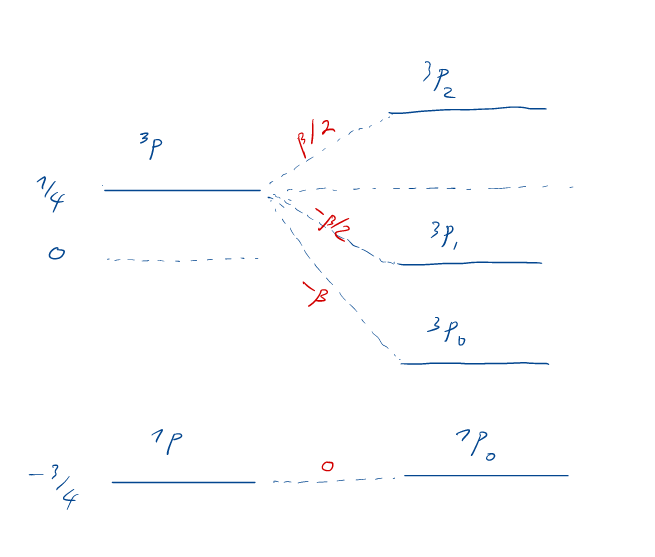
\includegraphics[width=0.61\textwidth]{levels_1.png}
	\end{figure}
	
	
	\newpage
	
	
	
	
	\item Now we will work in the regime where the spin exchange is a perturbation.  We wish to calculate the energy shifts due to $\be \gg 1$. To this end, we use perturbation theory to find the eigenenergies to first order in $\be$. But which basis do we use? We shall follow the hint and make a replacement 
	\begin{align*}
	\vec{s}_1 \cdot \vec{s}_2 \to \f{\langle \vec{s}_2 \cdot \vec{j}_2 \rangle}{\langle \vec{j}_2 \cdot \vec{j}_2\rangle} \vec{j}_1 \cdot \vec{j}_2
	\end{align*}
	where 
	\begin{align*}
	&\vec{j}_1 = \vec{l}_1 + \vec{s}_1 = \vec{s}_1\\
	&\vec{j}_2 = \vec{l}_2 + \vec{s}_2 .
	\end{align*}
	We may choose a basis in which $\vec{j}_1\cdot \vec{j}_2$ is diagonal. Let us call this basis $\ket{J m_J}$, where $\vec{J} = \vec{j}_1 + \vec{j}_2$. Here we have $j_1 = s_1 = 1/2$ and $j_2 =  1/2$ or $3/2$ since $l_2 = 1, s_2 = 1/2$.  If $j_2=1/2$, then $J=0$ or $J=1$. Let us first calculate the projection prefactor for $j_2=1/2$:
	\begin{align*}
	\f{\langle \vec{s}_2 \cdot \vec{j}_2 \rangle}{\langle \vec{j}_2 \cdot \vec{j}_2\rangle} 
	&= \f{\langle \vec{s}_2 \cdot (\vec{l}_2 + \vec{s}_2)\rangle }{j_2(j_2+1)}  \\
	&= \f{\langle s_2^2 + \vec{s}_2\cdot \vec{l}_2  \rangle }{j_2(j_2+1)}  \\
	&= \f{s_2(s_2+1) +(1/2)[j_2(j_2+1) - s_2(s_2+1) - l_2(l_2+1)]}{j_2(j_2+1)}\bigg\vert_{j_2=1/2,s_2=1/2,l_2 =1}\\
	&= -\f{1}{3}.
	\end{align*}
	Now we calculate $\vec{j}_1\cdot \vec{j}_2$ for various $J$ values with $j_2=1/2$:
	\begin{align*}
	&J=0: \quad\quad \f{1}{2}[J(J+1)-j_1(j_1+1)-j_2(j_2+1)]\bigg\vert_{J=0,j_1=1/2,j_2=1/2} =  -\f{3}{4}, \quad \text{1-degenerate} \\
	&J=1: \quad\quad \f{1}{2}[J(J+1)-j_1(j_1+1)-j_2(j_2+1)]\bigg\vert_{J=1,j_1=1/2,j_2=1/2} =  \f{1}{4},\quad \text{3-degenerate} 
	\end{align*}
	
	
	
	
	
	
	If $j_2=3/2$, then $J=1,2$. Let us first calculate the projection prefactor for $j_2=3/2$:
	\begin{align*}
	\f{\langle \vec{s}_2 \cdot \vec{j}_2 \rangle}{\langle \vec{j}_2 \cdot \vec{j}_2\rangle} 
	&= \f{\langle \vec{s}_2 \cdot (\vec{l}_2 + \vec{s}_2)\rangle }{j_2(j_2+1)}  \\
	&= \f{\langle s_2^2 + \vec{s}_2\cdot \vec{l}_2  \rangle }{j_2(j_2+1)}  \\
	&= \f{s_2(s_2+1) +(1/2)[j_2(j_2+1) - s_2(s_2+1) - l_2(l_2+1)]}{j_2(j_2+1)}\bigg\vert_{j_2=3/2,s_2=1/2,l_2 =1}\\
	&= \f{1}{3}.
	\end{align*}
	Now we calculate $\vec{j}_1\cdot \vec{j}_2$ for various $J$ values with $j_2=3/2$:
	\begin{align*}
	&J=1: \quad\quad \f{1}{2}[J(J+1)-j_1(j_1+1)-j_2(j_2+1)]\bigg\vert_{J=1,j_1=1/2,j_2=3/2} =  -\f{5}{4},\quad \text{3-degenerate} \\
	&J=2: \quad\quad \f{1}{2}[J(J+1)-j_1(j_1+1)-j_2(j_2+1)]\bigg\vert_{J=2,j_1=1/2,j_2=3/2} =  \f{3}{4}, \quad \text{5-degenerate}
	\end{align*}
	The result is that in the $j_2=1/2$ manifold the $J=0$ state shifts as $-\be + 1/4$, while the $J=1$ state shifts as $-\be -1/12$. In the $j_2=3/2$ manifold the $J=1$ state shifts as $\be/2 -5/12$, while the $J=2$ state shifts as $\be/2 + 1/4$. Figures \ref{fig:3} and \ref{fig:4} show how this manifests. 
	
	
	
	
	Of course, the new energy levels obey the sum rule: 
	\begin{align*}
	-\f{1}{3}\lb \textcolor{blue}{1}\times\lp \f{-3}{4}\rp + \textcolor{blue}{3}\times \f{1}{4} \rb + \f{1}{3}\lb \textcolor{blue}{3}\times\lp \f{-5}{4}\rp + \textcolor{blue}{5}\times \f{3}{4}  \rb = 0
	\end{align*}
	where the number in blue are the degeneracies for each $J$ state. 
	
	
	
	\begin{figure}[!htb]
		\centering
		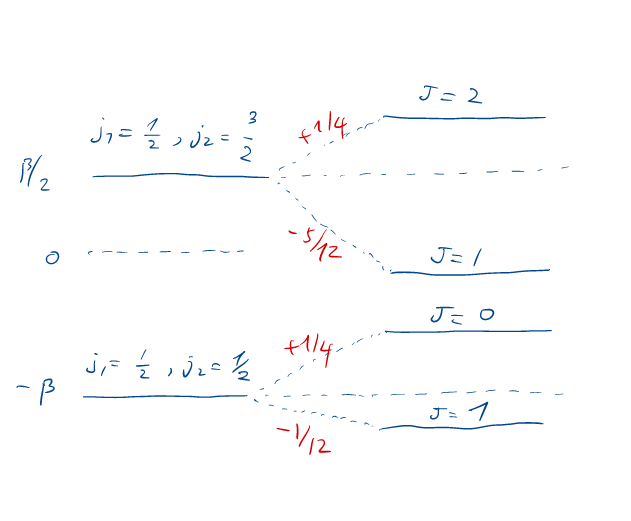
\includegraphics[width=0.7\textwidth]{levels_2.png}
	\end{figure}
	
	\newpage
	
	\item To obtain an exact solution for all field strengths, we shall work in the uncoupled basis $\ket{Lm_L s_1 m_{s_1} s_2 m_{s_2}}$. For short, let us write $\ket{m_L m_{s_1} m_{s_2}} = \ket{m_L \updownarrow\updownarrow}$. Here $L=1$ and $s_1 = s_2 = 1/2$, and so $m_L = \{-1,0,1\}$ and $m_{s_i} = \pm1/2$. The full Hamiltonian is 
	\begin{align*}
	\ham = \ham_\text{exch} + \ham_{\text{SO}} = \vec{s}_1 \cdot \vec{s}_2 + \be \vec{l}_2 \cdot \vec{s}_2.
	\end{align*}
	We shall evaluate the matrix elements of this Hamiltonian. This task seems a little daunting, but by breaking things down piece by piece it is only a matter of bookkeeping. First, let us evaluate the matrix elements associated with $\ham_\text{exch}$:
	\begin{align*}
	&\bra{m_{L} m_{s_1} m_{s_2} } \vec{s}_1 \cdot \vec{s}_2  \ket{m_{L}' m_{s_1}'  m_{s_2}'}\\
	&= \delta_{m_Lm_L'} \bra{m_{L} m_{s_1} m_{s_2} } s_{1z}s_{2z} + \f{1}{2}(s_1^+s_2^- + s_1^-s_2^+)  \ket{m_{L}' m_{s_1}'  m_{s_2}'} \\
	&= m_{s_1}'m_{s_2}' \delta_{m_Lm_L'} \delta_{m_{s_1}m_{s_1}'}\delta_{m_{s_2}m_{s_2}'}\\
	&\quad + \delta_{m_Lm_L'}\f{1}{2}\sqrt{s_1(s_1+1) - m_{s_1}'(m_{s_1}'+1)}\sqrt{s_2(s_2+1)-m_{s_2}'(m_{s_2}'-1)}\bra{m_L m_{s_1} m_{s_2}}\ket{m_L'(m_{s_1}'+1)(m_{s_2}'-1)}\\
	&\quad + \delta_{m_Lm_L'}\f{1}{2}\sqrt{s_1(s_1+1) - m_{s_1}'(m_{s_1}'-1)}\sqrt{s_2(s_2+1)-m_{s_2}'(m_{s_2}'+1)}\bra{m_L m_{s_1} m_{s_2}}\ket{m_L'(m_{s_1}'-1)(m_{s_2}'+1)}.
	\end{align*}
	There are only a few nonzero matrix elements. We note that the first summand gives elements along the diagonal. The value is 1/4 if $m_{s_1} = m_{s_2}$ and $-1/4$ if $m_{s_1} = -m_{s_2}$. The second summand takes the value $1/2$ if $m_{s_1}' = -1/2, m_{s_2}'=1/2$ and (thus) $m_{s_1} = 1/2, m_{s_2} = -1/2$, and zero otherwise. Similarly, the third summand takes the value $1/2$ if $m_{s_1}' = 1/2, m_{s_2}'= -1/2$ and (thus) $m_{s_1} = -1/2, m_{s_2} = 1/2$, and zero otherwise. The evaluation of the numerical prefactor is done by substituting the appropriate $m_{s_i}$ values and using $s_1= s_2 = 1/2$. With these, we are ready to write down $\ham_\text{exch}$ in our basis. 
	
	
	
	
	By ordering our 12-dimensional basis (left-to-right, top-to-bottom) as 
	\begin{align*}
	\{\ket{-1\downarrow\downarrow},
	\ket{-1\downarrow\uparrow},
	\ket{-1\uparrow\downarrow},
	\ket{-1\uparrow\uparrow},
	\ket{0\downarrow\downarrow},
	\ket{0\downarrow\uparrow},
	\ket{0\uparrow\downarrow},
	\ket{0\uparrow\uparrow},
	\ket{1\downarrow\downarrow},
	\ket{1\downarrow\uparrow},
	\ket{1\uparrow\downarrow},
	\ket{1\uparrow\uparrow}\}
	\end{align*}
	we obtain the following matrix for the $\ham_\text{exch}$:
	\begin{align*}
	\ham_\text{exch} = \begin{pmatrix}
	1/4 & & & \\
	& &-1/4 & 1/2 &\\
	& & 1/2 & -1/4 &\\
	& & & & 1/4
	\end{pmatrix} \oplus \begin{pmatrix}
	1/4 & & & \\
	& &-1/4 & 1/2 &\\
	& & 1/2 & -1/4 &\\
	& & & & 1/4
	\end{pmatrix}
	\oplus 
	\begin{pmatrix}
	1/4 & & & \\
	& &-1/4 & 1/2 &\\
	& & 1/2 & -1/4 &\\
	& & & & 1/4
	\end{pmatrix}
	\end{align*}
	where the $\oplus$ denotes the direct sum of the three $4\times 4$ summand matrices to make a 3-block-diagonal $12\times 12$ matrix. 
	
	
	To evaluate $\ham_{SO}$, we do the same thing really.  
	\begin{align*}
	&\be \bra{m_L m_{s_1} m_{s_2}} \vec{l}_2 \cdot \vec{s}_2 \ket{ m_L' m_{s_1}' m_{s_2}'} \\
	&= \be \delta_{m_{s_1}m_{s_1}'} \bra{m_L m_{s_1} m_{s_2}} L_z s_{2z} + \f{1}{2}(L^+s_2^- + L^- s_2^+)\ket{ m_L' m_{s_1}' m_{s_2}'} \\
	&= \be m_L'm_{s_2}' \delta_{m_L m_L'}\delta_{m_{s_1} m_{s_1}'}\delta_{m_{s_2} m_{s_2}'} \\
	&\quad + \f{\be}{2}\delta_{m_{s_1} m_{s_1}'}\sqrt{L(L+1)-m_L'(m_L'+1)}\sqrt{s_2(s_2+1)-m_{s_2}'(m_{s_2}'-1)} \bra{m_L m_{s_1}m_{s_2}}\ket{m_L'(m_L'+1) m_{s_1}'(m_{s_2}'-1)} \\
	&\quad + \f{\be}{2}\delta_{m_{s_1} m_{s_1}'}\sqrt{L(L+1)-m_L'(m_L'-1)}\sqrt{s_2(s_2+1)-m_{s_2}'(m_{s_2}'+1)} \bra{m_L m_{s_1}m_{s_2}}\ket{m_L'(m_L'-1) m_{s_1}'(m_{s_2}'+1)}.
	\end{align*}
	There are are only few nonzero matrix elements. The first summand contributes only to the diagonal. In our basis, the first summand gives
	\begin{align*}
	\ham_{\text{SO},1} =  \begin{pmatrix}
	\be/2 & & & \\
	& &-\be/2 &  &\\
	& & & \be/2 &\\
	& & & & -\be/2
	\end{pmatrix} \oplus \begin{pmatrix}
	 & & & \\
	& & &  &\\
	& & &  &\\
	& & & & 
	\end{pmatrix}
	\oplus 
	\begin{pmatrix}
	-\be/2 & & & \\
	& &\be/2 &  &\\
	& & & -\be/2 &\\
	& & & & \be/2
	\end{pmatrix}.
	\end{align*}
	The second summand takes the value of $1/\sqrt{2}$ whenever $m_{s_1} = m_{s_1}'$ with $(m_{s_2} = -1/2, m_{s_2}' = 1/2)$ and either $(m_L=1,m_L'=0)$ or $(m_L=0,m_L'=-1)$. Similarly, the third summand takes the value of $1/\sqrt{2}$ whenever $m_{s_1} = m_{s_1}'$ with $(m_{s_2} = 1/2, m_{s_2}' = -1/2)$ and either $(m_L=0,m_L'=1)$ or $(m_L=-1,m_L'=0)$. The evaluation of the numerical prefactor is done by substituting the appropriate $m$ values and using $L=1, s_1 = s_2 = 1/2$. The resulting $12\times 12$ matrix for $\ham_{SO}$ is 
	\begin{align*}
	\ham_{\text{SO}} = 
	\be\begin{pmatrix*}
	1/2 & 0 & 0 & 0 & 0 & 0 & 0 & 0 & 0 & 0 & 0 & 0 \\
	0 & -1/2 & 0 & 0 & 1/\sqrt{2} & 0 & 0 & 0 & 0 & 0 & 0 & 0 \\
	0 & 0 & 1/2 & 0 & 0 & 0 & 0 & 0 & 0 & 0 & 0 & 0 \\
	0 & 0 & 0 & -1/2 & 0 & 0 & 1/\sqrt{2} & 0 & 0 & 0 & 0 & 0 \\
	0 & 1/\sqrt{2} & 0 & 0 & 0 & 0 & 0 & 0 & 0 & 0 & 0 & 0 \\
	0 & 0 & 0 & 0 & 0 & 0 & 0 & 0 & 1/\sqrt{2} & 0 & 0 & 0 \\
	0 & 0 & 0 & 1/\sqrt{2} & 0 & 0 & 0 & 0 & 0 & 0 & 0 & 0 \\
	0 & 0 & 0 & 0 & 0 & 0 & 0 & 0 & 0 & 0 & 1/\sqrt{2} & 0 \\
	0 & 0 & 0 & 0 & 0 & 1/\sqrt{2} & 0 & 0 & -1/2 & 0 & 0 & 0 \\
	0 & 0 & 0 & 0 & 0 & 0 & 0 & 0 & 0 & 1/2 & 0 & 0 \\
	0 & 0 & 0 & 0 & 0 & 0 & 0 & 1/\sqrt{2} & 0 & 0 & -1/2 & 0 \\
	0 & 0 & 0 & 0 & 0 & 0 & 0 & 0 & 0 & 0 & 0 & 1/2 
	\end{pmatrix*}.
	\end{align*}
	Putting everything together, we find that
	\begin{align*}
	\ham = \left(
	\begin{array}{cccccccccccc}
	\frac{\beta }{2}+\frac{1}{4} & 0 & 0 & 0 & 0 & 0 & 0 & 0 & 0 & 0 & 0 & 0
	\\
	0 & -\frac{\beta }{2}-\frac{1}{4} & \frac{1}{2} & 0 & \frac{\beta
	}{\sqrt{2}} & 0 & 0 & 0 & 0 & 0 & 0 & 0 \\
	0 & \frac{1}{2} & \frac{\beta }{2}-\frac{1}{4} & 0 & 0 & 0 & 0 & 0 & 0 &
	0 & 0 & 0 \\
	0 & 0 & 0 & \frac{1}{4}-\frac{\beta }{2} & 0 & 0 & \frac{\beta
	}{\sqrt{2}} & 0 & 0 & 0 & 0 & 0 \\
	0 & \frac{\beta }{\sqrt{2}} & 0 & 0 & \frac{1}{4} & 0 & 0 & 0 & 0 & 0 &
	0 & 0 \\
	0 & 0 & 0 & 0 & 0 & -\frac{1}{4} & \frac{1}{2} & 0 & \frac{\beta
	}{\sqrt{2}} & 0 & 0 & 0 \\
	0 & 0 & 0 & \frac{\beta }{\sqrt{2}} & 0 & \frac{1}{2} & -\frac{1}{4} & 0
	& 0 & 0 & 0 & 0 \\
	0 & 0 & 0 & 0 & 0 & 0 & 0 & \frac{1}{4} & 0 & 0 & \frac{\beta
	}{\sqrt{2}} & 0 \\
	0 & 0 & 0 & 0 & 0 & \frac{\beta }{\sqrt{2}} & 0 & 0 &
	\frac{1}{4}-\frac{\beta }{2} & 0 & 0 & 0 \\
	0 & 0 & 0 & 0 & 0 & 0 & 0 & 0 & 0 & \frac{\beta }{2}-\frac{1}{4} &
	\frac{1}{2} & 0 \\
	0 & 0 & 0 & 0 & 0 & 0 & 0 & \frac{\beta }{\sqrt{2}} & 0 & \frac{1}{2} &
	-\frac{\beta }{2}-\frac{1}{4} & 0 \\
	0 & 0 & 0 & 0 & 0 & 0 & 0 & 0 & 0 & 0 & 0 & \frac{\beta }{2}+\frac{1}{4}
	\\
	\end{array}
	\right).
	\end{align*}
	Diagonalization is done in Mathematica. The distinct eigenvalues and their respective degeneracies are 
	\begin{align*}
	&E_0 = \f{-1}{4} \lp 1 + \be + \sqrt{4 + \be (-4 + 9 \be)}\rp, & \text{3-degenerate}\\
	&E_1 = \f{1}{4}-\be, & \text{1-degenerate}\\
	&E_2 = \f{-1}{4} \lp 1 + \be - \sqrt{4 + \be (-4 + 9 \be)}\rp, &\text{3-degenerate}\\
	&E_3 = \f{1}{4}(1+2\be), &\text{5-degenerate}.
	\end{align*}
	
	We can easily check in Mathematica that the sum rule still holds:
	\begin{align*}
	3E_0 + E_1 + 3E_2 + 5E_3 = 0.
	\end{align*}
	Another check is to calculate $\Tr(\ham)$. By inspection, we can see that it is zero. 
	
	
	
	
	
	
	
	Finally, let us check this result against our approximations in the low and high field limits. To this end, we shall plot the eigenvalues as a function of $\be$. Figure \ref{fig:1} shows how the unperturbed $^1P_0$ and $^3P_{0,1,2}$ levels split in the presence of low $\be\neq 0$. Figure \ref{fig:2} shows the overall behavior at high $\be$.  Figures \ref{fig:3} and \ref{fig:4} are zoomed-in versions of Figure \ref{fig:2}. We see good agreement in both regimes. 
	
	
	\begin{figure}[!htb]
		\centering
		\includegraphics[width=0.8\textwidth]{B_low.eps}
		\caption{Energies as a function of $\be$ at low fields. The black dashed lines are our predictions from part (c), which agree well with exact diagonalization of the Hamiltonian.}
		\label{fig:1}
	\end{figure}


	At high fields, we have that the two limiting eigenenergies are $E_- = -\be$ and $E_+ = \be/2$. These are shown as the black dashed lines in Figure \ref{fig:2}.  Figures \ref{fig:3} and \ref{fig:4} zoom into each limit and let us to see how the splittings of each manifold agree with our prediction in part (d). 


	\begin{figure}[!htb]
		\centering
		\includegraphics[width=0.8\textwidth]{B_high.eps}
		\caption{Energies as a function of $\be$ at high fields. The black dashed lines show the high field limits. }
		\label{fig:2}
	\end{figure}

	
		
	\begin{figure}[!htb]
		\centering
		\includegraphics[width=0.8\textwidth]{B_high_zoom_1.eps}
		\caption{The $j_2=3/2$ manifold at high fields. The purple lines are predictions from part (d). The upper purple dashed line is the $J=2$ state, the lower purple dashed line is the $J=1$ state. The black dashed line is the "center" energy level of the $j_2=3/2$ manifold in the presence of strong $\be$. The $J$ states are shifted from this by constants.} 
		\label{fig:3}
	\end{figure}
	
	
	\begin{figure}[!htb]
		\centering
		\includegraphics[width=0.8\textwidth]{B_high_zoom_2.eps}
		\caption{The $j_2=1/2$ manifold at high fields. The purple lines are predictions from part (d). The upper purple dashed line is the $J=1$ state, the lower purple dashed line is the $J=0$ state. The black dashed line is the "center" energy level of the $j_2=1/2$ manifold in the presence of strong $\be$. The $J$ states are shifted from this by constants.} 
		\label{fig:4}
	\end{figure}
	
\end{enumerate}


\end{document}








